\documentclass[12pt]{article}\usepackage[]{graphicx}\usepackage[]{color}
%% maxwidth is the original width if it is less than linewidth
%% otherwise use linewidth (to make sure the graphics do not exceed the margin)
\makeatletter
\def\maxwidth{ %
  \ifdim\Gin@nat@width>\linewidth
    \linewidth
  \else
    \Gin@nat@width
  \fi
}
\makeatother

\definecolor{fgcolor}{rgb}{0.345, 0.345, 0.345}
\newcommand{\hlnum}[1]{\textcolor[rgb]{0.686,0.059,0.569}{#1}}%
\newcommand{\hlstr}[1]{\textcolor[rgb]{0.192,0.494,0.8}{#1}}%
\newcommand{\hlcom}[1]{\textcolor[rgb]{0.678,0.584,0.686}{\textit{#1}}}%
\newcommand{\hlopt}[1]{\textcolor[rgb]{0,0,0}{#1}}%
\newcommand{\hlstd}[1]{\textcolor[rgb]{0.345,0.345,0.345}{#1}}%
\newcommand{\hlkwa}[1]{\textcolor[rgb]{0.161,0.373,0.58}{\textbf{#1}}}%
\newcommand{\hlkwb}[1]{\textcolor[rgb]{0.69,0.353,0.396}{#1}}%
\newcommand{\hlkwc}[1]{\textcolor[rgb]{0.333,0.667,0.333}{#1}}%
\newcommand{\hlkwd}[1]{\textcolor[rgb]{0.737,0.353,0.396}{\textbf{#1}}}%
\let\hlipl\hlkwb

\usepackage{framed}
\makeatletter
\newenvironment{kframe}{%
 \def\at@end@of@kframe{}%
 \ifinner\ifhmode%
  \def\at@end@of@kframe{\end{minipage}}%
  \begin{minipage}{\columnwidth}%
 \fi\fi%
 \def\FrameCommand##1{\hskip\@totalleftmargin \hskip-\fboxsep
 \colorbox{shadecolor}{##1}\hskip-\fboxsep
     % There is no \\@totalrightmargin, so:
     \hskip-\linewidth \hskip-\@totalleftmargin \hskip\columnwidth}%
 \MakeFramed {\advance\hsize-\width
   \@totalleftmargin\z@ \linewidth\hsize
   \@setminipage}}%
 {\par\unskip\endMakeFramed%
 \at@end@of@kframe}
\makeatother

\definecolor{shadecolor}{rgb}{.97, .97, .97}
\definecolor{messagecolor}{rgb}{0, 0, 0}
\definecolor{warningcolor}{rgb}{1, 0, 1}
\definecolor{errorcolor}{rgb}{1, 0, 0}
\newenvironment{knitrout}{}{} % an empty environment to be redefined in TeX

\usepackage{alltt}

%%% PAGE DIMENSIONS
\usepackage{geometry}
\geometry{a4paper}
\geometry{margin=2cm}

%%% PACKAGES
\usepackage[authoryear]{natbib}
\bibliographystyle{besjournals}

\usepackage{makecell,booktabs}

\usepackage{setspace}
\doublespacing
% \linespread{1.25}

\usepackage{graphicx}

\usepackage{tabularx}
\usepackage{adjustbox}

\usepackage{multirow}

\usepackage[running]{lineno}

\usepackage{caption}
\captionsetup{justification=raggedright, singlelinecheck=false}
\usepackage[font=small,labelfont=bf,labelsep=space]{caption}

\usepackage{subcaption}
\captionsetup{justification=raggedright, singlelinecheck=false}
\usepackage[font=small,labelfont=bf,labelsep=space]{subcaption}

\usepackage{pgfplots}
\pgfplotsset{width=16cm}

\usepackage{authblk}

\usepackage{amsmath}

\usepackage{hyperref} % for \url

\usepackage{pdflscape} %for landscape table

\usepackage{afterpage} %for Table on next page

%%% HEADERS and FOOTERS
\usepackage{fancyhdr}
\pagestyle{fancy}
\renewcommand{\headrulewidth}{0pt}
\lhead{}\chead{}\rhead{}
\lfoot{}\cfoot{\thepage}\rfoot{}

%%% SECTION TITLE APPEARANCE
\usepackage{sectsty}
\setcounter{secnumdepth}{-1}
\subsectionfont{\normalfont\fontsize{14}{15}\selectfont}
\DeclareMathSizes{10}{11}{9}{7}

%%% DEFINE NEW COMMANDS
\newcommand{\B}{\textbf}
\newcommand{\TL}{\textless}
\newcommand{\PRZ}{\text{Pr}\bigl( >\mid Z \mid \bigr)}
\newcommand{\head}[1]{\textnormal{\textbf{#1}}}

\newenvironment{nscenter}
 {\parskip=.75pt\par\nopagebreak\centering}
 {\par\noindent\ignorespacesafterend}

\makeatletter
\renewcommand{\fnum@figure}{Fig. \thefigure.}
\renewcommand{\fnum@table}{Table \thetable.}
\makeatother

\newcommand{\fillcaption}[1]{ %new command with the argument being the text of the caption
\textbf{Fig. \arabic{figure}:} #1 %Makes main figure number, concatenates it to legend
\addtocounter {figure} {1} %increments main figure count
}

%% FOR SUPPLEMENT SETTINGS
\newcommand{\beginsupplement}{%
        \setcounter{table}{0}
        \renewcommand{\thetable}{S\arabic{table}}%
        \setcounter{figure}{0}
        \renewcommand{\thefigure}{S\arabic{figure}}%
     }
\IfFileExists{upquote.sty}{\usepackage{upquote}}{}
\begin{document}
\linenumbers

%%% DOCUMENT CONTENT
\title{Decoupling plant economics traits and biomass carbon composition in wetland litter \\ \huge Supplemental Material}
\author[*ab]{S. M. Windecker}
\author[b]{S. M. Trevathan-Tackett}
\author[a]{N. Golding}
\author[acd]{J. A. Catford}
\author[b]{P. I. Macreadie}
\author[a]{P. A. Vesk}

\affil[a]{School of BioSciences, University of Melbourne, Parkville VIC 3010, Australia}
\affil[b]{Centre for Integrative Ecology, School of Life and Environmental Sciences, Deakin University, Burwood Campus, Burwood VIC 3125, Australia}
\affil[c]{Biological Sciences, University of Southampton, Highfield Campus, Southampton SO17 1BJ, UK}
\affil[d]{Fenner School of Environment and Society, Australian National University, Canberra ACT 2601, Australia}
\affil[*]{Corresponding author: sm.windecker@unimelb.edu.au}
\date{}
\maketitle

\pgfplotsset{width=16cm}

\begin{figure}[!ht]
	\scalebox{0.5}
	{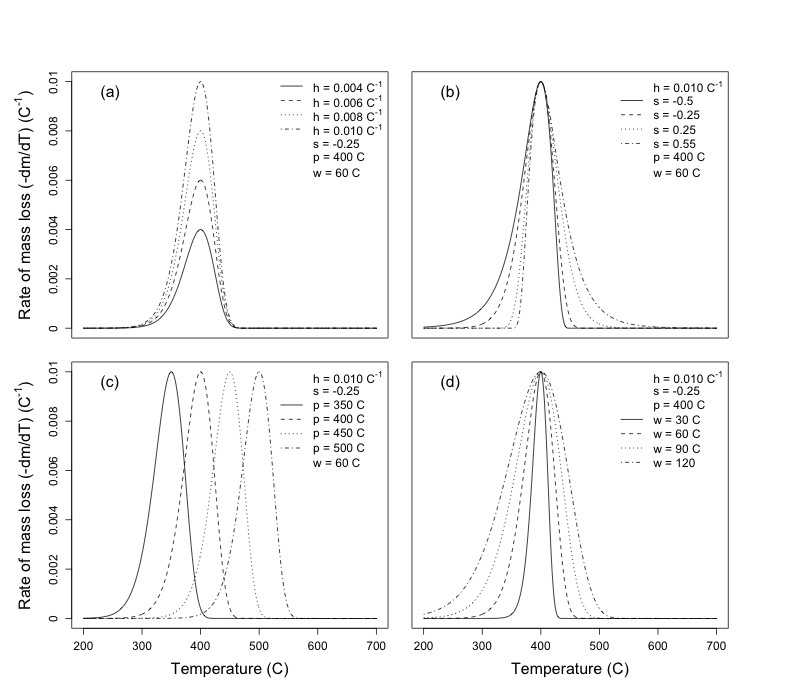
\includegraphics{figs/fs_simulate.png}}
	\caption{Parametric study of the Fraser-Suzuki function for deconvolution of derivative thermogravimetric biomass curves: (a) Effect of modifying height; (b) skew; (c) position; and (d) width.}
	\label{Fig:fs_simulation}
\end{figure}

\afterpage{%
	\clearpage%
	\thispagestyle{empty}
	\begin{landscape}%
	\centering
		\begin{table}[!htbp]
		\caption{Fraser-Suzuki mixture model parameter estimates for each species.}
		\label{Tab:parameters}
		\begin{adjustbox}{width=1.5\textwidth}
		\begin{tabular}{l r r r r r r r r r r r r r r r r}
		\toprule
		\multicolumn{1}{c}{} & \multicolumn{4}{l}{Height} & \multicolumn{4}{l}{Position} & \multicolumn{4}{l}{Skew} & \multicolumn{4}{l}{Width}\\
		\cmidrule(lr){2-5}
		\cmidrule(lr){6-9}
		\cmidrule(lr){10-13}
		\cmidrule(lr){14-17}
		Species & HC-1 & HC-2 & CL & LG & HC-1 & HC-2 & CL & LG & HC-1 & HC-2 & CL & LG & HC-1 & HC-2 & CL & LG \\
		\midrule
		 Acacia dealbata &  NA & 1.36e-03 & 2.25e-03 & 2.42e-03 &  & 265 & 316 & 330 &  & -0.22 & -0.33 & 0.08 &  & 53.00 & 32.20 & 217 \\ 
  Alternanthera denticulata &  NA & 1.68e-03 & 3.24e-03 & 1.36e-03 &  & 233 & 308 & 330 &  & 0.13 & -0.14 & 0.25 &  & 86.90 & 50.00 & 224 \\ 
  Baumea articulata &  NA & 3.68e-03 & 7.24e-03 & 1.07e-03 &  & 263 & 317 & 330 &  & -0.01 & -0.23 & 0.17 &  & 55.50 & 27.40 & 250 \\ 
  Baumea rubiginosa &  NA & 3.89e-03 & 6.04e-03 & 1.01e-03 &  & 266 & 320 & 330 &  & 0.25 & -0.07 & 0.25 &  & 57.80 & 26.40 & 250 \\ 
  Carex appressa &  NA & 3.37e-03 & 6.81e-03 & 1.05e-03 &  & 268 & 321 & 330 &  & -0.12 & -0.17 & 0.11 &  & 57.00 & 27.40 & 250 \\ 
  Carex fascicularis &  NA & 2.53e-03 & 5.55e-03 & 1.02e-03 &  & 265 & 319 & 330 &  & -0.33 & -0.27 & 0.18 &  & 56.80 & 30.50 & 250 \\ 
  Crassula helmsii &  NA & 2.61e-03 & 1.59e-03 & 1.17e-03 &  & 280 & 311 & 330 &  & -0.25 & -0.26 & 0.25 &  & 50.00 & 50.00 & 250 \\ 
  Cycnogeton procerum &  NA & 1.62e-03 & 3.39e-03 & 1.48e-03 &  & 250 & 308 & 330 &  & -0.33 & -0.33 & -0.10 &  & 50.00 & 30.90 & 250 \\ 
  Cyperus eragrostis & 1.57e-03 & 2.65e-03 & 4.47e-03 & 8.64e-04 & 194 & 269 & 311 & 330 & -0.32 & 0.00 & -0.20 & 0.20 & 33.10 & 90.00 & 27.00 & 250 \\ 
  Eleocharis acuta &  NA & 2.42e-03 & 5.73e-03 & 1.22e-03 &  & 270 & 319 & 330 &  & -0.08 & -0.06 & 0.07 &  & 56.10 & 29.70 & 250 \\ 
  Eucalyptus camaldulensis &  NA & 1.41e-03 & 2.18e-03 & 2.04e-03 &  & 251 & 324 & 369 &  & -0.28 & -0.33 & -0.17 &  & 100.00 & 29.60 & 203 \\ 
  Gahnia filum &  NA & 3.98e-03 & 7.22e-03 & 1.04e-03 &  & 280 & 311 & 330 &  & -0.30 & -0.24 & 0.25 &  & 50.20 & 27.70 & 250 \\ 
  Juncus amabilis &  NA & 3.95e-03 & 5.80e-03 & 1.16e-03 &  & 266 & 317 & 330 &  & 0.12 & 0.01 & 0.09 &  & 51.00 & 28.70 & 250 \\ 
  Juncus procerus &  NA & 2.89e-03 & 4.47e-03 & 1.22e-03 &  & 269 & 322 & 330 &  & 0.22 & 0.05 & 0.10 &  & 65.50 & 27.90 & 250 \\ 
  Lycopus australis &  NA & 1.79e-03 & 3.57e-03 & 1.46e-03 &  & 264 & 312 & 330 &  & -0.33 & -0.30 & 0.25 &  & 73.00 & 47.80 & 217 \\ 
  Marsilea drummondii & 8.30e-04 & 2.50e-03 & 3.84e-03 & 1.16e-03 & 188 & 274 & 316 & 330 & -0.20 & -0.33 & -0.14 & 0.20 & 54.50 & 50.00 & 33.60 & 250 \\ 
  Melaleuca ericifolia &  NA & 1.67e-03 & 2.23e-03 & 1.76e-03 &  & 268 & 334 & 330 &  & 0.25 & -0.23 & 0.10 &  & 72.90 & 29.70 & 250 \\ 
  Melaleuca squarrosa & 1.87e-04 & 1.23e-03 & 2.13e-03 & 2.46e-03 & 153 & 262 & 338 & 330 & 0.20 & 0.16 & -0.20 & 0.20 & 80.00 & 61.30 & 30.30 & 200 \\ 
  Meuhlenbeckia florulenta & 2.58e-04 & 2.42e-03 & 4.30e-03 & 1.21e-03 & 143 & 270 & 326 & 358 & -0.16 & -0.01 & -0.12 & 0.20 & 80.00 & 74.90 & 34.90 & 230 \\ 
  Myriophyllum crispatum & 8.19e-04 & 2.29e-03 & 2.69e-03 & 1.04e-03 & 210 & 259 & 313 & 389 & -0.33 & 0.02 & -0.05 & 0.20 & 80.00 & 58.20 & 32.30 & 213 \\ 
  Nymphaea alba &  NA & 1.82e-03 & 2.50e-03 & 1.34e-03 &  & 234 & 310 & 330 &  & -0.33 & -0.33 & 0.11 &  & 65.30 & 44.40 & 250 \\ 
  Paspalum distichum &  NA & 3.24e-03 & 4.83e-03 & 8.50e-04 &  & 275 & 316 & 344 &  & -0.33 & -0.29 & 0.03 &  & 50.00 & 50.00 & 250 \\ 
  Persicaria decipiens &  NA & 2.58e-03 & 2.71e-03 & 1.12e-03 &  & 280 & 325 & 332 &  & -0.33 & -0.33 & 0.25 &  & 60.10 & 43.10 & 250 \\ 
  Persicaria prostrata &  NA & 2.66e-03 & 3.23e-03 & 1.18e-03 &  & 272 & 314 & 330 &  & -0.33 & -0.11 & 0.25 &  & 70.20 & 37.00 & 250 \\ 
  Phragmites australis &  NA & 2.96e-03 & 6.10e-03 & 1.26e-03 &  & 265 & 321 & 330 &  & 0.14 & -0.18 & 0.11 &  & 59.50 & 27.90 & 250 \\ 
  Restio tetraphyllus &  NA & 4.07e-03 & 5.75e-03 & 1.17e-03 &  & 266 & 330 & 330 &  & 0.25 & -0.10 & 0.25 &  & 50.50 & 30.10 & 250 \\ 
  Rumex crispus &  NA & 1.78e-03 & 2.49e-03 & 1.20e-03 &  & 244 & 296 & 347 &  & -0.33 & 0.13 & 0.10 &  & 79.30 & 34.90 & 250 \\ 
  Sphagnum sp &  NA & 2.69e-03 & 4.14e-03 & 1.15e-03 &  & 280 & 331 & 333 &  & 0.20 & -0.31 & 0.25 &  & 61.60 & 40.40 & 250 \\ 
  Typha domingensis &  NA & 2.03e-03 & 6.25e-03 & 1.38e-03 &  & 270 & 324 & 330 &  & -0.03 & -0.29 & 0.01 &  & 66.30 & 22.70 & 250 \\ 
  
		\bottomrule
		\end{tabular}
		\end{adjustbox}
	\end{table}
\end{landscape}
\clearpage
}

\begin{table}[ht] \centering
	\caption{GenBank Accession codes.}
	\label{Tab:genbank}
	\begin{tabular}{l l l}
	\toprule
		Species & rbcl & matK \\
		\midrule
		\input{figs/gen_bank_accessions.tex}
		\bottomrule
	\end{tabular}
\end{table}

\afterpage{%
	\clearpage%
	\thispagestyle{empty}
	\begin{landscape}%
	\centering
	\begin{figure}
	\scalebox{0.4}
	{\includegraphics{figs/phylo_all.png}}
	\caption{Phylogenetic tree of species with traits. Tree at genus level where species level sequences for rcbL gene unavailable. If the branch represents more than one species, the trait value was averaged among species in that genus.}
	\label{Fig:phylo}
\end{figure}
\end{landscape}
\clearpage
}

\begin{table}[ht]
  \centering
	\caption{Mantel test for the correlation between branch length distance and functional trait distances between the seven traits.}
	\label{Tab:mantel}
	\begin{tabular}{l r r}
	\toprule
		Trait & Mantel Test observation & $P$-value \\
		\midrule
		 \textbf{Specific litter area} & \textbf{0.42} & \textbf{0.01} \\ 
  Litter dry matter content & 0.06 & 0.26 \\ 
  Litter nitrogen & -0.1 & 0.71 \\ 
  Litter carbon & -0.13 & 0.85 \\ 
  Litter hemicelluloses & -0.11 & 0.83 \\ 
  Litter cellulose & -0.01 & 0.47 \\ 
  Litter lignin & -0.14 & 0.87 \\ 
  
		\bottomrule
	\end{tabular}
\end{table}

\begin{figure}[!ht]
	\scalebox{0.3}
	{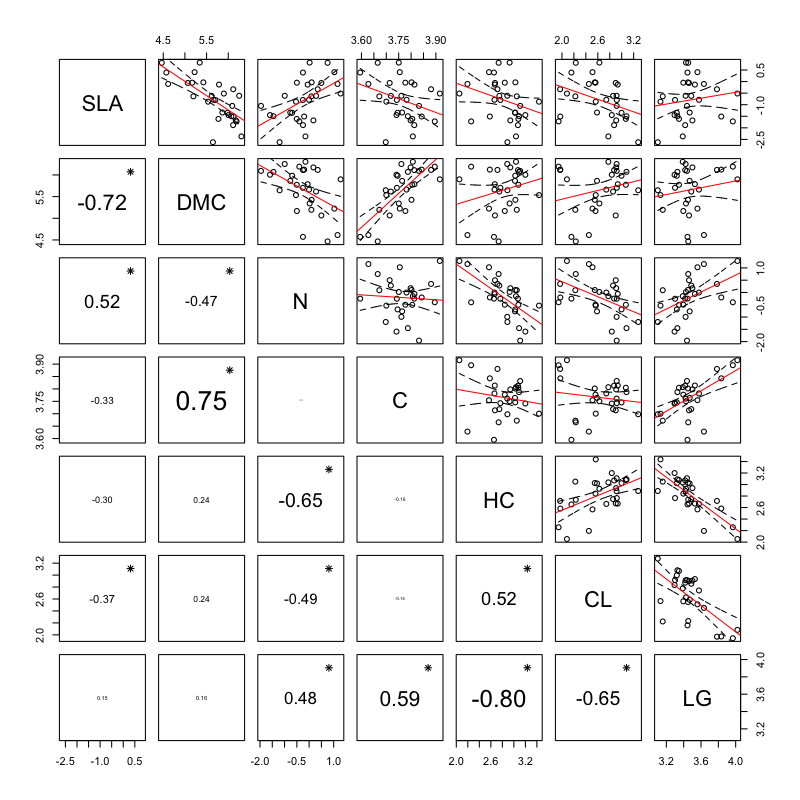
\includegraphics{figs/pairplot.png}}
	\caption{Correlations between traits. Size of $R^2$ listed on bottom panel proportional to weight of relationship, with star to indicate significance at P \textless 0.05.}
	\label{Fig:pairplot}
\end{figure}

\begin{figure}[!ht]
\centering
	\begin{subfigure}[ht]{0.9\textwidth}
		\includegraphics[width=\textwidth]{figs/tga_ar.png}
		\subcaption{DTG deconvolution for amphibious fluctuation-responders (n = 5).}
		\label{Fig:tga_ar}
	\end{subfigure}\hfill
\end{figure}
\begin{figure}[!ht]\ContinuedFloat
	\begin{subfigure}[ht]{0.9\textwidth}
		\includegraphics[width=\textwidth]{figs/tga_at.png}
		\subcaption{DTG deconvolution for amphibious fluctuation-tolerators (n = 11).}
		\label{Fig:tga_at}
	\end{subfigure}\hfill
\end{figure}
\begin{figure}[!ht]\ContinuedFloat
	\begin{subfigure}[ht]{0.9\textwidth}
		\includegraphics[width=\textwidth]{figs/tga_tda.png}
		\subcaption{DTG deconvolution for terrestrial damp species (n = 8).}
		\label{Fig:tga_tda}
	\end{subfigure}\hfill
\end{figure}
\begin{figure}[!ht]\ContinuedFloat
	\begin{subfigure}[ht]{0.9\textwidth}
		\includegraphics[width=\textwidth]{figs/tga_tdr.png}
		\subcaption{DTG deconvolution for terrestrial dry species (n = 5).}
		\label{Fig:tga_tdr}
	\end{subfigure}
	\caption{All species first derivative thermogravimetric (DTG) deconvolutions: (a) amphibious fluctuation-responders; (b) amphibious fluctuation-tolerators; (c) terrestrial damp species; and (d) terrestrial dry species.}
	\label{Fig:tga_all}
\end{figure}

\begin{table}[!htbp]\centering
	\caption{Principal Component Analysis axis loadings.}
	\label{Tab:pca}
	\begin{tabular}{l r r r r}
        		\toprule
        		Trait & Axis 1 & Axis 2 \\
        		\midrule
		 Specific litter area & 0.37 & 0.34 \\ 
  Litter dry matter content & -0.29 & -0.54 \\ 
  Litter nitrogen & 0.47 & 0.07 \\ 
  Litter carbon & 0.00 & -0.61 \\ 
  Litter hemicelluloses & -0.47 & 0.17 \\ 
  Litter cellulose & -0.43 & 0.12 \\ 
  Litter lignin & 0.40 & -0.43 \\ 
  
        		\bottomrule
	\end{tabular}
\end{table}

\afterpage{%
	\clearpage%
	\thispagestyle{empty}
	\begin{landscape}%
	\centering
\begin{table}[ht]
	\caption{Hierarchical classification scheme of wetland plant species by habit and response to water. Devised by Brock and Casanova (1997).}
	\label{Tab:fxl_groups}
	\centering
	\small
	\begin{tabularx}{\textwidth}{lllX}
        		\toprule
        		Abbreviation & Primary category & Secondary category & Description \\
        		\midrule
		AR & Amphibious & Fluctuation-responders & Species which germinate in flooded conditions, grow in both flooded and damp conditions, and reproduce above the surface of the water. \\
		AT & Amphibious & Fluctuation-tolerators & Species which germinate in damp or flooded conditions and tolerate variation in water level. \\
		Tda & Terrestrial & Damp species & Species which germinate, grow, and reproduce on saturated soil. \\
		Tdr & Terrestrial & Dry species & Species which germinate, grow, and reproduce where there is no surface water and water table is below the soil surface. \\
        		\bottomrule
	\end{tabularx}
\end{table}
\end{landscape}
\clearpage
}

\begin{figure}
	\centering
	\scalebox{0.3}
	{\includegraphics{figs/tga_pure_samples.png}}
	\caption{Predicted negative derivative thermogravimetric for raw biomass samples: (a) carboxy-methyl cellulose; (b) alkali lignin.}
	\label{Fig:tga_pure}
\end{figure}


\end{document}
